\chapter{مشخصات یک پایان نامه و گزارش علمی}
\section{مقدمه}
در این فصل، عملکرد مدل \lr{ProActionCLIP} در زمینه‌ی یادگیری پیوسته‌ی تشخیص حرکت انسان مورد ارزیابی قرار می‌گیرد. هدف از این ارزیابی، بررسی میزان صحت مدل در یادگیری وظایف جدید، ارزیابی میزان فراموشی دانش پیشین و تحلیل بهره‌وری محاسباتی آن از نظر مصرف سخت‌افزار و تعداد پارامترهای قابل‌آموزش است. به منظور ارزیابی جامع، مدل پیشنهادی با روش‌های مطرح در این حوزه مانند \lr{PIVOT} \cite{pivot}و سایر رویکردهای مرجع مقایسه می‌شود. برای این منظور، از مجموعه‌داده‌های نظیر \lr{UCF101} \cite{ucf101} و \lr{HMDB51} \cite{hmdb51} استفاده شده است.

در ادامه‌ی‌ این فصل، ابتدا معیارهای ارزیابی شامل صحت، میزان فراموشی معرفی می‌شوند. سپس، جزئیات مربوط به مجموعه‌های داده، تنظیمات آزمایشی، روش‌های مقایسه‌ای و تحلیل نتایج ارائه خواهد شد تا ارزیابی مدل پیشنهادی به‌طور کامل و شفاف صورت گیرد. در اخر نیز پیچیدگی محاسباتی بررسی خواهد شد. 
% سخت افزار رو تو همون پیچیدگی محاسباتی بگم. پارامتر. شامل حافظه . بگم رو جی پی یو فلان اموزش دادم. 

\section{معیار‌های ارزیابی}
در یادگیری پیوسته، دو معیار ارزیابی اهمیت دارند. یکی از آن‌ها میانگین صحت وظایف با وجود یادگیری سایر وظایف بوده و دیگری میزان فراموشی مدل پس از یادگیری هر وظیفه است که در ادامه هر یک شرح داده خواهد شد. 
 

\subsection{میانگین صحت}
در یادگیری پیوسته، عملکرد مدل روی تمام وظایف یادگرفته شده تاکنون توسط میانگین صحت ارزیابی می‌گردد. دو نوع صحت $top1$ و $top5$ در این تحقیق بررسی می‌شود. صحت $top1$ بیان‌گر این است که پیش‌بینی‌کننده، از بین احتمالات بدست آمده، برچسب با بیشترین احتمال را انتخاب می‌کند و سپس برابر بودن آن با برچسب واقعی داده‌ی بررسی‌شده، سنجیده می‌‌شود. اما در صحت $top5$، پنج تا برچسب با بیشترین احتمال، انتخاب شده و وجود یا عدم وجود برچسب واقعی در این پنج برچسب بررسی می‌شود. مطابق با \eqref{eq:acc_top_1} و \eqref{eq:acc_top_5}، میانگین صحت در وظیفه‌ی فعلی، برای همین وظیفه و وظایف قبلی، در حالت $top1$ و $top5$ بدست می‌آید. $\text{\lr{ACC}}^{top1}_{i,t}$ نشانگر صحت $top1$ برای وظیفه‌ی $i$ بعد از یادگیری وظیفه‌ی $t$ و $\text{\lr{ACC}}^{top5}_{i,t}$ نشانگر صحت $top5$ برای وظیفه‌ی $i$ بعد از یادگیری وظیفه‌ی $t$ می‌باشد.
\begin{equation}\label{eq:acc_top_1}
	A_{top1}(t) = \frac{1}{t+1} \sum_{i=0}^{t} \text{\lr{ACC}}^{top1}_{i,t}
\end{equation}
\begin{equation}\label{eq:acc_top_5}
	A_{top5}(t) = \frac{1}{t+1} \sum_{i=0}^{t} \text{\lr{ACC}}^{top5}_{i,t}
\end{equation}

\subsection{میزان فراموشی}
در یادگیری پیوسته، مدل باید بتواند وظایف جدید را یاد بگیرد بدون اینکه دانش وظایف قبلی را فراموش کند. اما معمولاً پدیده‌ی فراموشی فاجعه‌آمیز رخ می‌دهد؛ یعنی مدل پس از یادگیری وظایف جدید، صحت آن روی وظایف قدیمی کاهش پیدا می‌کند. معیار فراموشی برای اندازه‌گیری میزان این افت عملکرد تعریف می‌شود و به صورت میانگین کاهش دقت در وظایف قبلی است. بر اساس \eqref{eq:forget_task_i}، فراموشی مدل روی وظیفه‌ی $i$ پس از یادگیری وظیفه‌ی $t$ بدست می‌آید. ماتریس \lr{ACC}، شامل صحت مدل روی هر وظیفه پس از یادگیری همان وظیفه و وظیفه‌های دیگر است. به دنبال آن، $\text{\lr{ACC}}_{i,k}$ نشان‌دهنده‌ی صحت مدل روی وظیفه‌ی $i$ پس از یادگیری وظیفه‌ی $k$ است. به این ترتیب، اختلاف بین بیشترین صحتی که وظیفه‌ی $i$ پس از یادگیری وظایف مختلف بدست آورده و صحتی که پس از وظیفه‌ی $t$ (آخرین وظیفه‌ی یادگرفته شده) بدست آمده، در $f_i(t)$ قرار می‌گیرد. در نهایت فراموشی برای هر وظیفه محاسبه شده و میانگین آن‌ها به عنوان فراموشی مدل پس از یادگیری وظیفه‌ی $t$، در نظر گرفته می‌شود (\eqref{eq:forget_final}). 
\begin{equation}\label{eq:forget_task_i}
	f_i(t) = \max_{k \le t} \text{\lr{ACC}}_{i,k} - \text{\lr{ACC}}_{i,t}
\end{equation}
\begin{equation}\label{eq:forget_final}
	F(t) = \frac{1}{t} \sum_{i=1}^{t} f_i(t) 
\end{equation}

\section{مجموعه‌داده}
در این تحقیق از دو مجموعه‌داده‌ی مرسوم تشخیص حرکت با نام‌های \lr{UCF101}\cite{ucf101} و \lr{HMDB51} \cite{hmdb51} استفاده شده است که در ادامه هریک شرح داده خواهد شد. 

\subsection{مجموعه‌داده‌ی \lr{UCF101}}
مجموعه‌داده‌ی \lr{UCF101} \cite{ucf101} یکی از مجموعه‌داده‌های استاندارد و پرکاربرد در زمینه تشخیص حرکات انسانی در ویدیو است. 
این مجموعه شامل \lr{13{,}320} ویدیو از \lr{101} دسته‌ی مختلف فعالیت انسانی است که طیف وسیعی از حرکات روزمره، ورزشی و تعاملی را پوشش می‌دهد. 
نمونه‌های این مجموعه‌داده از ویدیوهای واقعی و متنوع جمع‌آوری شده‌اند و شامل تغییرات قابل توجه در شرایط نور، پس‌زمینه، زاویه دید و ظاهر اشخاص هستند.
\begin{figure}
	\centering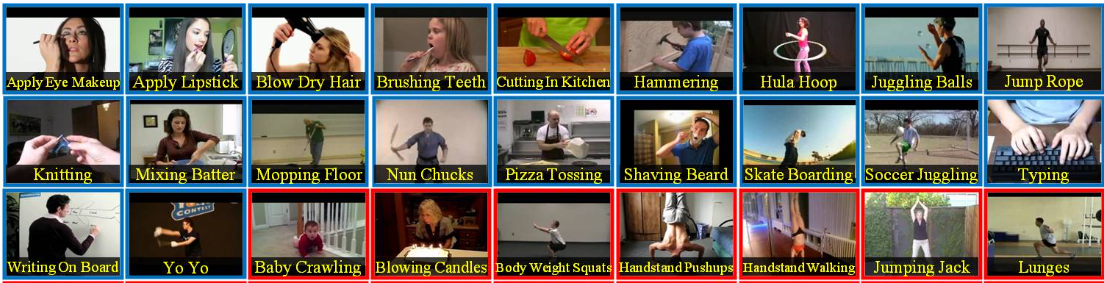
\includegraphics[scale=.5]{Images/Chapter4/ucf101.png}
	\caption[]{ نمونه‌ای از مجموعه‌داده‌ی \lr{UCF101}\cite{ucf101}   }
	\label{fig.41}
\end{figure}
دسته‌های موجود در \lr{UCF101} به پنج گروه کلی تقسیم می‌شوند:
\begin{enumerate}
	\item \textbf{‌فعالیت‌های ورزشی} 
	\item \textbf{فعالیت‌های تعاملی انسان با اشیا} 
	\item \textbf{فعالیت‌های تعاملی انسان با انسان} 
	\item \textbf{فعالیت‌های بدنی عمومی} 
	\item \textbf{فعالیت‌های نواختن موسیقی} 
\end{enumerate}

ویژگی مهم این مجموعه‌داده، تنوع بالای آن در شرایط تصویربرداری و پیچیدگی حرکات است 
که آن را به یک معیار معتبر برای ارزیابی مدل‌های تشخیص حرکات‌های انسانی و یادگیری پیوسته تبدیل می‌کند. نمونه‌هایی از داده‌های این مجموعه‌داده در \cref{fig.41} قابل مشاهده است. 
‌\subsection{مجموعه‌داده‌ی \lr{HMDB51}}
مجموعه‌داده \lr{HMDB51} \cite{hmdb51} یکی از مجموعه‌داده‌های پرکاربرد در زمینه‌ی تشخیص حرکات انسانی در ویدیو است که برای ارزیابی عملکرد الگوریتم‌های تشخیص حرکت طراحی شده است. 
این مجموعه شامل \lr{6{,}766} ویدیو در \lr{51} دسته‌ی فعالیت انسانی است که هر دسته تقریباً ۱۰۰ نمونه دارد. 
نمونه‌های موجود در \lr{HMDB51} از منابع متنوعی همچون فیلم‌های سینمایی، ویدیو‌های اینترنتی و فیلم‌های خانگی جمع‌آوری شده‌اند 
و طیف وسیعی از حرکات انسانی شامل فعالیت‌های بدنی، تعامل انسان با اشیاء و تعامل انسان با انسان را پوشش می‌دهند. یکی از ویژگی‌های مهم این مجموعه‌داده، تنوع بالا در صحنه، پس‌زمینه، زاویه دوربین و کیفیت ویدیوها است 
که تشخیص حرکات را به یک چالش واقعی تبدیل می‌کند. 
\begin{figure}
	\centering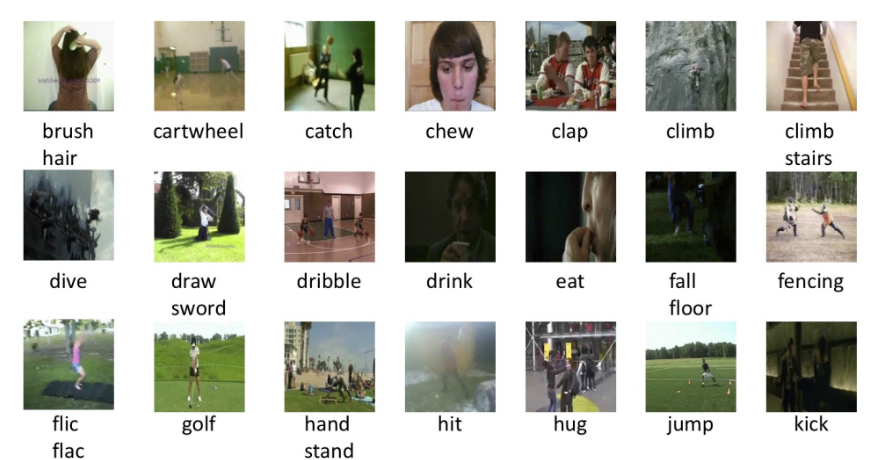
\includegraphics[scale=.6]{Images/Chapter4/HMDB_snapshot1-300x225.png}
	\caption[]{ نمونه‌ای از مجموعه‌داده‌ی \lr{HMDB51}\cite{hmdb51}   }
	\label{fig.42}
\end{figure}
به دلیل اندازه متوسط و تنوع مناسب، \lr{HMDB51} به‌طور گسترده برای آموزش و ارزیابی مدل‌های تشخیص حرکات و یادگیری پیوسته مورد استفاده قرار می‌گیرد. فعالیت‌های موجود در \lr{HMDB51} را می‌توان در پنج گروه کلی دسته‌بندی کرد:
\begin{enumerate}
	\item \textbf{فعالیت‌های عمومی صورت}
	\item \textbf{فعالیت‌های صورت همراه با تعامل با اشیا} 
	\item \textbf{حرکات عمومی بدن} 
	\item \textbf{حرکات بدن همراه با تعامل با اشیا} 
	\item \textbf{حرکات بدن در تعامل انسان با انسان} 
\end{enumerate}
نمونه‌ای از این داده‌ها در \cref{fig.42} قابل مشاهده است.
\section{تنظیمات آزمایش}








